
\section{Methods}
\label{sec:methods}
\subsection{Data}\label{sec:data}

Our primary datasets are the TREC 2013/2014 Stream Corpus, 
a ?tb corpus of hourly 
web crawls from October 2011
through mid February 2013
\cite{frank2012building}.\footnote{\url{http://trec-kba.org/kba-stream-corpus-2014.shtml}}
%KM - Keep neutral from Trec
%As per the TS specifications,
All summary sentences come from processing this
corpus in a time aligned manner.
%KM - Are you using both 2013 and 2014 corpora.
%KM - Mentioning sentence ids at this point is too low level.
%KM - I would probably just drop this sentence. since you say above that you
%use both.
%While the 2014 corpus encompasses the 
%2013 corpus, we use the 2013 corpus for evaluating events from the 2013 track
%year because sentence ID's used in evaluation changed from year to year.



\subsubsection{Events}

%KM - You said this already so I think you can make it simpler. 
%We use the event set developed for the TREC Temporal Summarization track 
%for years 2013 and 2014.
The TREC 2013 and 2014 Stream corpus contains  10 and 15 events respectively. We omit
one event from the 2013 track because there were no news documents in the 
corpus during the duration of the event, yielding a final event set of 24 
events. Meta-data provided for each event includes the name of the event
as it appears on Wikipedia, a short text query for the event, 
the type of event, and the 
duration of the event.
%KM - the below parens is not clear. is ``to monitor'' missing from the above
%sentence? I think get rid of the parens below.
%(the duration for the system 
%to monitor is not necessarily the complete timespan of the event).
%KM - Let's get rid of all references to ``the TS system'' If you want to have
%a system name, choose a better one. 
All data except the Wikipedia name is exposed to
systems that participate in TREC.
%the TS system to use.

\subsubsection{Wikipedia}

\kmcomment{
 As far as I can see this is the first time you've mentioned this.
 This paragraph is not clearly understandable. Is this the training data?
 Also confusing here is that you alternate between what TREC provides and
 what you do. This absolutely must be clear. Are these wikipedia pages provided
 by TREC or do you create a wikipedia corpus on your own?}

For each event type we identified one or more related Wikipedia
categories and collected all pages that were listed under that category for use
as training data.
For all pages collected, we used the latest possible revision date before the
start of the Stream Corpus. 

We use the  Wikipedia corpora to construct the language models used
in our salience prediction model (\cref{subsubsec:lm}). For each of the five
event types shown in Fig.~\ref{fig:wikipedia}, we used all data in the pages
shown to build a language model. The amount of words per event type varied from
6 million to 250 million.
\kmcomment{moved this to the end since it is less of a priority}
We used the same corpus to train our semantic similarity component
(\cref{subsec:semsim}. 
Disaster specific term-sentence matrices were built using subsections of
Wikipedia.
\kmcomment{I don't think you ever mention term-sentence matrices earlier.}
\begin{figure*}
        \begin{center}
\begin{tabular}{| p{5cm} c c |}
\hline
Event & WP Categories & No. Docs/Sents/Words\\
\hline \hline
2012 Aurora shooting \newline
Wisconsin Sikh temple shooting\newline 
2012 Tel Aviv bus bombing \newline
Boston\_Marathon\_bombings \newline
Christopher\_Dorner\_shootings\_and\_manhunt \newline 
 In\_Amenas\_hostage\_crisis
& Terrorism, Mass Shootings & 33,732/1,139,588/26,201,659  \\
\hline
Hurricane Isaac (2012) \newline
Hurricane Sandy \newline
Typhoon Bopha \newline
2012 Guatemala earthquake \newline
 Cyclone\_Oswald \newline
Early\_2012\_European\_cold\_wave \newline
February\_2013\_noreaster \newline & Natural Disasters & 35,554/591,850/12,794,438  \\
\hline
2012 Buenos Aires Rail Disaster
2012 Pakistan garment factory fires
Costa\_Concordia\_disaster & Accidents & 22,874/732,945/16,520,242 \\
\hline
Chelyabinsk\_meteor & Astronomy & 14,515/283,509/6,135,803  \\
\hline
Port\_Said\_Stadium\_riot \newline
2012\_Afghanistan\_Quran\_burning\_protests \newline
2011-13\_Russian\_protests \newline
2012\_Romanian\_protests \newline
2012-13\_Egyptian\_protests \newline
2013\_Bulgarian\_protests\_against\_the\_Borisov\_cabinet \newline
2013\_Shahbag\_protests & Activism\_by\_type & 464,657/11,254,122/250,172,896  \\
\hline
\end{tabular}
\caption{Domain specific Wikipedia corpora for semantic similarity and 
language models. }
\label{fig:wikipedia}
\end{center}
\end{figure*} 



\subsubsection{Nuggets}
For evaluation purposes, important pieces of information, hereafter 
referred to as nuggets, were extracted from each event's Wikipedia page.
%KM - What assessors? Was this done by TREC? Make clear. I added ``TREC'' after
%reading ahead.
%KM - What do you mean ``graded''? Do you mean they graded your nuggets? Or do
%you mean they ``ranked'' the nuggets by importance. Please make clear.
TREC assessors graded nuggets by importance, and were also able to timestamp
%KM - wrong wording. I've changed.
%their
%existance
the occurrence time of the events represented by each nugget
using the timestamp of the page's revision history. Nuggets are 
usually a short to medium length clause containing an atomic piece of
information.
%KM - I think an example of a nugget here could help.

\kmcomment{ I changed title to make clearer}
\subsubsection{Gold Standard} %Matches}

A gold standard dataset consisting of full sentences from the TREC datastream
was constructed to use for scoring of the system we describe here. It would be
difficult to automatically match full sentences against the nuggets identified
by TREC assessors given the substantial difference in length; each nugget
typically appears as a clause or phrase in the sentence.

TREC assessors provided judgements on a subset of participant updates (i.e.,
full sentences)  each year
of the track. Judged updates are matched to one or more nuggets (a real 
sentence often contains more than one atomic piece of information) or marked
not relevant.

%KM - I don't see why overlap in particpant update sets would give you low
%coverage. In fact, it might you give you broader coverage than if all
%participants extracted the same sentences.  I removed first portion of the
%sentence, but you can put back and clarify if you think I interpreted
%incorrectly. 
%There was not much overlap in the participant update sets so
Overall coverage of
%KM - Shouldn't this be nuggets?
%relevant sentences
relevant nuggets in the corpus  by participant systems' generated sentences
is small (percent?). Thus we augmented the pool of previous participant system
output with judgments on new system output using Amazon Mechanical Turk. For
each sentence produced by our system and by our baselines, we asked turkers to
indicate which of the nuggets were conveyed by the sentence. For each hit, we
provided one sentence and five nuggets. For each nugget, they had to answer a
yes-no question indicating whether it was conveyed by the full sentence.
%KM - This is complicated. More explanation is needed.
%KM - The sentence below sounds like how you evaluate your system and not like
%the judgment corpus.
%KM not sure this owuld go here. Shouldn't it go in evaluation? Here you would
%just talk about the corpus
To evaluate new system output on the same event, we compare it against the
corpus of matched sentences. Comparing it against the nuggets would not yield
meaningful results as the nuggets are much smaller than the sentences of the
corpus.
%KM - Let's discuss where these different things go. I think scoring should
%probably go in the evaluation section.
\kmcomment{I think this sentence should go in the evaluation section. This
  subsection is about data.}
Because there are so few matched sentences, we score all new system updates as positive
%To expand the judgement corpora, we include all system updates as positive
nugget matches if they are $< .2$ close in Levenshtein distance to a human
assessed matched update. 

\subsection{Experiment Design}

\subsubsection{Salience Models}
For each event (both in the complete system and feature ablation experiments)
we randomly sample 1000 sentences after relevant document filtering and 
over the duration of the event 
as determined by 
TREC; avgerage run length is ? days.
%KM - Should you say here using the sentence similarity software? 
Nugget similarities
are computed for each sentence and are standardized with respect to 
the sample mean and variance. After standardization, the maximum nugget
similarities are computed for each sentence.
%KM - I think it would be helpful to mention that you use the features below
%here. 
We fit a Gaussian process for each event, using the maximum similarities 
as our regression target, yielding 24 models in total. Kernel lengthscale
parameters are also individually fit for each model.
%KM - Do you mean for new events? Would help if you say so. 
When making event-specific predictions, we take the average prediction of the
23 other models.

\subsubsection{Estimating Language Models}
We use two trigram language models, trained using the SRILM toolkit
\cite{stolcke2002srilm}, taking as features the average log probability (i.e.
the sentence's total log probability normalized by sentence length) from each
model.  This first model is trained on 4 years (2005-2009) of articles from the
Gigaword corpus.  Specifically, we use articles from the Associated Press and
the New York Times. The second model is a domain specific language model.
%KM - Remind us how many event types there are. Do you list all at some point?
We build a corpus of Wikipedia articles for each event type, consisting of documents from a related Wikipedia category. E.g. for earthquakes, we collect pages under the category \emph{Category:Earthquakes}. This model assigns higher probability to sentences that are focused on the given domain.

% For each event, we retrieve all sentences using the document retrieval and content selection steps outlined in the previous selection. We then sample with replacement 200 sentences from this collection, and extract non-lexical features for each sentence to construct our design matrix $\mathbf{X}$. To build our response variables $\mathbf{y}$ we compute the maximum semantic similarity of each input sentence to the gold nugget sentences. We fit a $\operatorname{GP}$ with an RBF kernel to this data, optimizing kernel parameters with the scaled  conjugate gradient method. This sampling procedure is repeated 100 times for each of the ? 2013 TS events, yielding \fdcomment{?} total models. In our salience predictions for the 2014 events, we take the mean prediction of all models.


\subsubsection{Redundancy Threshold}

For every time interval with input, a clustering algorithm is
guarranteed to produce at least one output; 
this can significantly hurt the performance of all clustering based 
temporal summarization systems. In order to avoid this, we set a threshold $t$
such that a new update must have a maximum similarity $< t$ to all previous 
updates.

We determined the value of $t$ by examining the distribution of similarities
of nuggets to their human-matched sentences compared to the distribution
of similarities of nuggets to relevant but non matching sentences. We fit
normal distributions for the matching and non-matching similarities and
used the point of intersection as the value of $t$.
%KM _ I think you need to say here what sentence similarity method you use.
%Just saying ``cosine similarity'' implies word overlap.
Figure ? shows a normalized histogram of cosine similarities for both 
distributions, the fitted distributions, and the point of intersection.

\begin{figure}
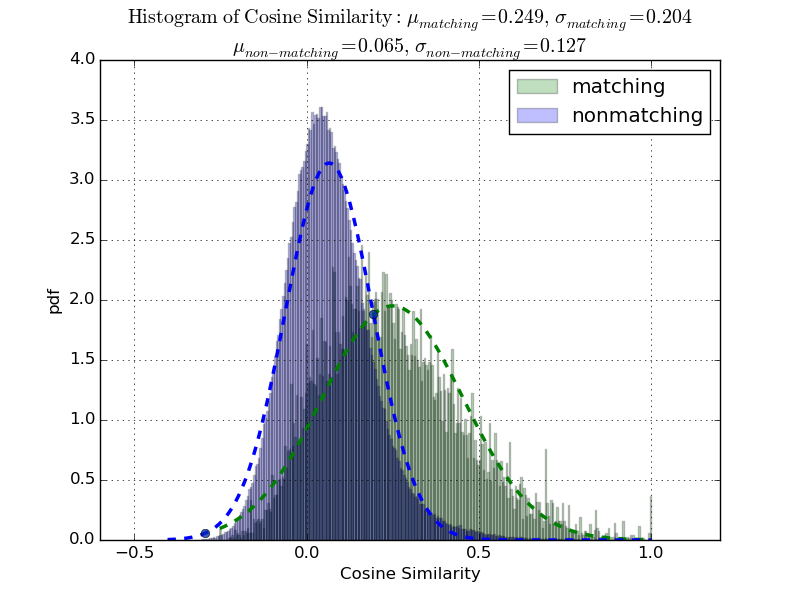
\includegraphics[scale=.40]{match-dist.png} 
\caption{Distribution of nugget similarity for matching and non-matching 
updates.\fdcomment{possible to output this as a vector graphic (pdf pref).  it will scale better.}}
\end{figure}

%KM _ What happened to the geo-codes? Aren't they in the salience models?
\subsubsection{Effect of Salience Models}

In order to assess the effectiveness of the salience predictions on update
selection, we perform a baseline (AP-base) run using affinity propagation 
clustering
with uniform preference, i.e. all preferences are equal to the median sentence
similarity. This run is compared to our full system (AP-sal), using each
sentence's salience prediction as its preference. 

%KM - I think this should be rewritten to say you compare to a usual
%summarization technique, using hierarchical agglomerative clustering with
%selection of sentences at the centroid of the cluster.
%We are also interested
%in the effect of directly incorporating salience in the clustering algorithm.
%A third run (HAC) is performed using hierarchical agglomerative 
%clustering; we produce flattened clusters by setting a maximum cluster 
%distance threshold. The sentence with the highest predicted salience from each
% cluster is selected as an update. 
%The distance threshold was tuned using grid search. By comparing
%HAV with AP-base we can empirically assess the trade off between preference
%and neighbor similarity that affinity propagation is making.
%KM - I now see why you were running experiments this way. It would be an
%interesting test.

%KM - Here is a paragraph you could use. I commented out above but you can put
%back in if there are pieces you prefer. Of course, edit below any way you see
%fit. Probably cite Radev and Jing here. They did this fairly early. There may
%be others who did this later.

We also compared our system against a typical summarization approach using
hierarchical agglomerative clustering (HAC); we produce flattened clusters by setting a maximum cluster 
distance threshold. We  select the centroid of each
cluster as a summary sentence  \cite{??}. 

\subsubsection{Feature Ablation}

%KM - Probably should describe this as either backward search over feature
%groups. There's a word for this. I will find it. Also should start with the
%purpose of doing it. 
We remove each feature group and train models models on these small 
feature subsets. All other parameters are the same as in our full system 
(AP-sal).



